% ---------------------------------------------------------------------------
% Realtime Programming -- single source for lecture script AND slides
%
% MODE SWITCH: choose ONE of the two lines below (or override on the command
% line, see Makefile:  make script | make slides).
% ---------------------------------------------------------------------------
\providecommand{\lecturemode}{script}   % <-- change to: slides   (or script)

\RequirePackage{etoolbox}
\newtoggle{slides}
\ifdefstring{\lecturemode}{slides}{\toggletrue{slides}}{\togglefalse{slides}}

\iftoggle{slides}{%
  \documentclass[aspectratio=169,10pt]{beamer}
  \usetheme{metropolis}
}{%
  \documentclass[a4paper,11pt]{scrartcl}
  \usepackage{beamerarticle}
  \usepackage[margin=2.5cm]{geometry}
}

\usepackage[utf8]{inputenc}
\usepackage[T1]{fontenc}
\usepackage{lmodern}
\usepackage{amsmath}
\usepackage{booktabs}
\usepackage{tikz}
\usetikzlibrary{arrows.meta,positioning,calc}
\usepackage{listings}
\usepackage{xcolor}
\usepackage{url}

\lstdefinestyle{arduino}{
  language=C++,
  basicstyle=\ttfamily\footnotesize,
  keywordstyle=\color{blue!70!black},
  commentstyle=\color{green!40!black},
  numbers=left, numberstyle=\tiny\color{gray},
  breaklines=true, columns=fullflexible, keepspaces=true,
  frame=single, rulecolor=\color{gray!50},
}
\lstset{style=arduino}

% Text that appears only in the script (long-form explanation)
\newcommand{\scriptonly}[1]{\iftoggle{slides}{}{#1}}
% Text that appears only on slides
\newcommand{\slidesonly}[1]{\iftoggle{slides}{#1}{}}

% Wokwi example: include sketch from examples/<dir>/sketch.ino
\newcommand{\wokwiexample}[3]{% dir, caption, label
  \lstinputlisting[caption={#2},label={#3}]{examples/#1/sketch.ino}%
}


\title{Realtime Programming}
\subtitle{Lecture \iftoggle{slides}{slides}{script}}
\author{Prof.\ Dr.\ Markus Pfeil}
\date{\today}

\begin{document}

\iftoggle{slides}{%
  \frame{\titlepage}%
  \begin{frame}{Outline}\tableofcontents\end{frame}%
}{%
  \maketitle
  \tableofcontents
  \newpage
}

\section{Realtime Concepts}

\subsection{Definitions}
\begin{frame}{What is realtime?}
  \begin{itemize}
    \item Realtime computing: hardware and software systems subject to a \emph{realtime constraint}, i.e.\ an operational deadline from event to system response.
    \item A computation \emph{fails} if it is not completed before its deadline.
    \item The deadline must be met \emph{regardless of system load}.
    \item Fast is not the same as realtime: a fast system without a guaranteed deadline is not a realtime system.
  \end{itemize}
\end{frame}

\scriptonly{%
Realtime does not mean ``as fast as possible''. It means that the correctness of a result depends on \emph{when} it is delivered, not only on its value. A braking controller that calculates the right brake force 200\,ms too late is wrong.
}

\subsection{Time conditions}
\begin{frame}{Time conditions}
  \begin{itemize}
    \item \textbf{Exact time}: an action at $t_0$.
    \item \textbf{Deadline}: no later than $t_{max}$.
    \item \textbf{Earliest time}: not before $t_{min}$.
    \item \textbf{Interval}: between $t_{min}$ and $t_{max}$.
    \item \textbf{Periodic}: at $k\cdot t_s$, $k = 0,1,2,\dots$
    \item \textbf{Non-periodic}: at $t_1, t_2, t_3,\dots$ (e.g.\ driven by external events)
  \end{itemize}
\end{frame}

\subsection{Hard and soft realtime}
\begin{frame}{Hard and soft realtime}
  \begin{description}
    \item[Hard] Time conditions must be met, otherwise catastrophic failure. A deviation is a serious error.
    \item[Soft] Deadlines should be met, with some tolerance: averages, or a statistical distribution of response times.
    \item[Concurrency] Realtime systems handle several inputs and outputs at the same time.
  \end{description}
\end{frame}

\subsection{Processing time and load}
\begin{frame}{Response time and load}
  \begin{center}
  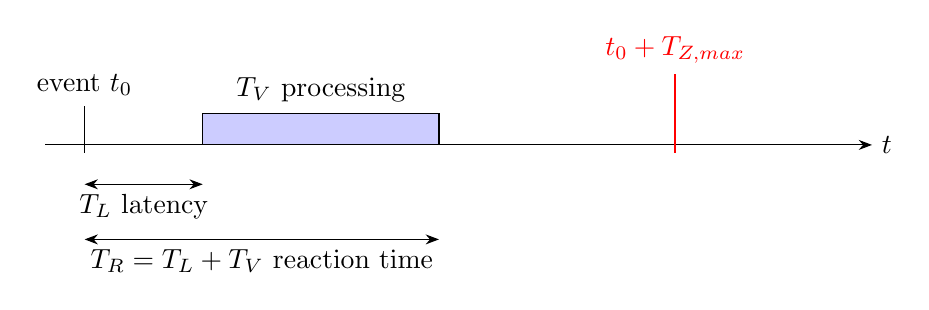
\begin{tikzpicture}[x=1cm,y=1cm,>=Stealth]
    \draw[->] (0,0) -- (10.5,0) node[right] {$t$};
    \draw (0.5,-0.1) -- (0.5,0.5) node[above] {event $t_0$};
    \draw[fill=blue!20] (2,0) rectangle (5,0.4);
    \node at (3.5,0.7) {$T_V$ processing};
    \draw[<->] (0.5,-0.5) -- (2,-0.5) node[midway,below] {$T_L$ latency};
    \draw[<->] (0.5,-1.2) -- (5,-1.2) node[midway,below] {$T_R = T_L + T_V$ reaction time};
    \draw[red,thick] (8,-0.1) -- (8,0.9) node[above] {$t_0 + T_{Z,max}$};
  \end{tikzpicture}
  \end{center}
  \begin{align*}
    T_V = \frac{N}{P}, \qquad \rho = \frac{T_V}{T_P} < 1
  \end{align*}
  Requirement: $T_R \le T_{Z,max}$.
\end{frame}

\scriptonly{%
$N$ is the number of operations, $P$ the computing power in operations per second, $T_P$ the time between two requests of the same type. The utilisation $\rho = T_V/T_P$ must always be smaller than~1. Latency $T_L$ is the time the task waits before it starts, for example because another task or an interrupt is running. In a realtime system the \emph{maximum} of $T_R$ is what counts, not the average.
}

\subsection{Where to measure: WCET}
\begin{frame}{Why measure timing?}
  \begin{itemize}
    \item Realtime guarantees need the \emph{worst-case execution time} (WCET) of every task.
    \item The WCET can be analysed statically or measured externally.
    \item In this lecture: toggle a GPIO pin at start and end of a code section and record it with a \textbf{logic analyzer} (Chapter~\ref{sec:timing}).
  \end{itemize}
\end{frame}

\section{Tasks in FreeRTOS}

\subsection{Task functions}
\begin{frame}{Task functions}
  \begin{itemize}
    \item A task is a C function: \texttt{void aTask(void *pvParameters)}.
    \item It has an entry point and normally runs forever in an infinite loop.
    \item It must never \texttt{return}. If it is no longer needed, delete it with \texttt{vTaskDelete()}.
    \item Every task has its \emph{own stack} and its own copy of local variables.
    \item One function can be used to create several tasks.
  \end{itemize}
\end{frame}

\subsection{Creating tasks}
\begin{frame}[fragile]{Creating tasks}
\begin{lstlisting}
BaseType_t xTaskCreate(
    TaskFunction_t pvTaskCode,   // the task function
    const char *pcName,          // name (debugging)
    uint16_t usStackDepth,       // stack size in words
    void *pvParameters,          // passed to the task
    UBaseType_t uxPriority,      // 0 = lowest
    TaskHandle_t *pxCreatedTask);// handle (may be NULL)
\end{lstlisting}
\end{frame}

\subsection{Task states}
\begin{frame}{Task states}
  \begin{center}
  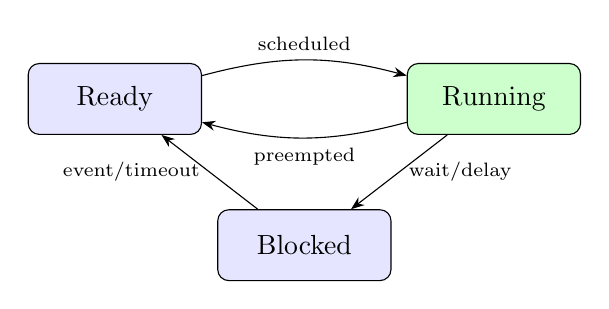
\begin{tikzpicture}[node distance=2.6cm,>=Stealth,
      st/.style={draw,rounded corners,minimum width=2.2cm,minimum height=0.9cm,fill=blue!10}]
    \node[st] (ready) {Ready};
    \node[st,right=of ready,fill=green!20] (run) {Running};
    \node[st,below=1.4cm of $(ready)!0.5!(run)$] (block) {Blocked};
    \draw[->] (ready) to[bend left=15] node[above]{\scriptsize scheduled} (run);
    \draw[->] (run) to[bend left=15] node[below]{\scriptsize preempted} (ready);
    \draw[->] (run) -- node[right]{\scriptsize wait/delay} (block);
    \draw[->] (block) -- node[left]{\scriptsize event/timeout} (ready);
  \end{tikzpicture}
  \end{center}
  Plus \emph{Suspended} (via \texttt{vTaskSuspend()}). Only Ready tasks compete for the CPU.
\end{frame}

\subsection{Priorities and the scheduler}
\begin{frame}{Priority-based preemptive scheduling}
  \begin{itemize}
    \item Priorities $0 \dots$ \texttt{configMAX\_PRIORITIES}$-1$, higher number = higher priority.
    \item The scheduler always runs the highest-priority Ready task.
    \item Tasks with equal priority share the CPU in round-robin time slices.
    \item Time slices are based on the \emph{tick} interrupt. On this AVR port the tick comes from the watchdog timer: 15\,ms.
  \end{itemize}
\end{frame}

\scriptonly{%
Internally, FreeRTOS keeps one ready list per priority level (\texttt{pxReadyTasksLists[]}). On a context switch, \texttt{vTaskSwitchContext()} walks down from the highest priority with a non-empty list and takes the next entry of that list. Because the list is circular, tasks of the same priority get equal shares. These few lines are the core of the scheduler; the rest of the kernel exists to keep them correct.
}

\subsection{Blocking and periodic tasks}
\begin{frame}{Delaying: \texttt{vTaskDelay} vs.\ \texttt{vTaskDelayUntil}}
  \begin{itemize}
    \item \texttt{vTaskDelay(n)}: block for $n$ ticks \emph{after the call}. Period = execution time + delay $\Rightarrow$ drift.
    \item \texttt{vTaskDelayUntil(\&last, n)}: block until \texttt{last + n}. Fixed period, independent of the execution time.
    \item A blocked task uses no CPU. The \emph{idle task} runs when nothing else is Ready.
  \end{itemize}
\end{frame}

\subsection{Example}
\begin{frame}[fragile]{Wokwi example 1: two tasks, two priorities}
  \wokwiexample{ex01_tasks_priorities}{Two periodic tasks, traced by the scheduler}{lst:ex01}
\end{frame}

\scriptonly{%
Example~\ref{lst:ex01} creates two periodic tasks. The patched scheduler sets the trace pin of a task high while it is Running and low otherwise. Attach a logic analyzer to pins 10 and 11 (see Chapter~\ref{sec:timing}) to see when each task runs and how the higher-priority task preempts the other.
}

\section{Synchronization}

\subsection{Semaphores}
\begin{frame}{Semaphores: signalling between tasks and ISRs}
  \begin{itemize}
    \item A \emph{binary semaphore} signals an event: one side \texttt{Give}s, the other \texttt{Take}s.
    \item The waiting task is \emph{Blocked}, uses no CPU, and becomes Ready when the semaphore is given.
    \item ISRs use \texttt{xSemaphoreGiveFromISR()} and defer the real work to a task (``deferred interrupt processing'').
    \item \emph{Counting semaphores} count events or manage a pool of resources.
  \end{itemize}
\end{frame}

\begin{frame}[fragile]{Wokwi example 2: ISR $\rightarrow$ semaphore $\rightarrow$ task}
  \wokwiexample{ex02_isr_semaphore}{Button interrupt wakes a task}{lst:ex02}
\end{frame}

\scriptonly{%
Keep the ISR short: it gives the semaphore and requests a context switch if a higher-priority task was woken. The latency from the button edge to the first instruction of the task is exactly the kind of timing we measure in Chapter~\ref{sec:timing}.
}

\subsection{Mutexes and priority inversion}
\begin{frame}{Semaphore vs.\ mutex}
  \begin{itemize}
    \item \textbf{Semaphore}: signalling. Different tasks give and take.
    \item \textbf{Mutex}: protects a shared resource. The same task takes and gives, always in this order.
    \item Both are implemented on top of queues in FreeRTOS.
  \end{itemize}
\end{frame}

\begin{frame}{Priority inversion and inheritance}
  \begin{itemize}
    \item Low task $L$ holds a mutex, high task $H$ waits for it, medium task $M$ preempts $L$ $\Rightarrow$ $H$ is blocked by $M$ for an unbounded time.
    \item \textbf{Priority inheritance}: $L$ temporarily inherits $H$'s priority while $H$ waits. FreeRTOS mutexes do this; binary semaphores do not.
  \end{itemize}
\end{frame}

\subsection{Deadlocks}
\begin{frame}{Deadlocks}
  \begin{itemize}
    \item Two or more tasks are blocked forever, each waiting for a resource held by another.
    \item Avoidance: acquire resources in a fixed global order, use timeouts, keep critical sections short.
  \end{itemize}
\end{frame}

\section{Queues}

\begin{frame}{Queues}
  \begin{itemize}
    \item Primary means of inter-task communication, also usable from ISRs.
    \item Items are \emph{copied} into the queue (deep copy), so the sender's variable can go out of scope.
    \item For large items, queue a pointer instead.
    \item Sending and receiving can block with a timeout: the blocked task is put on the queue's \emph{waiting to send/receive} list and does not consume CPU.
  \end{itemize}
\end{frame}

\begin{frame}[fragile]{Queue API}
\begin{lstlisting}
QueueHandle_t q = xQueueCreate(8, sizeof(int));

xQueueSend(q, &value, pdMS_TO_TICKS(10));    // block <= 10 ms
xQueueReceive(q, &value, portMAX_DELAY);     // block forever
xQueueSendFromISR(q, &value, &woken);        // inside an ISR
\end{lstlisting}
\end{frame}

\begin{frame}[fragile]{Wokwi example 3: producer and consumer}
  \wokwiexample{ex03_queue}{Producer/consumer with a queue}{lst:ex03}
\end{frame}

\scriptonly{%
The consumer blocks on the queue until an item arrives. If the consumer has the higher priority it runs immediately after each send. If the producer has the higher priority, the queue fills up and the producer blocks on a full queue. Use the logic analyzer to observe both cases.
}

\section{Scheduling and Schedulability}

\subsection{Periodic tasks}
\begin{frame}{Periodic tasks and processor demand}
  Task $i$: period $T_i$, execution time $C_i$, implicit deadline $D_i = T_i$.
  \[ U_i = \frac{C_i}{T_i}, \qquad U = \sum_i U_i \]
  \begin{itemize}
    \item Example: $T_1 = 200$\,ms, $C_1 = 100$\,ms $\Rightarrow$ 50\,\%; $T_2 = 100$\,ms, $C_2 = 50$\,ms $\Rightarrow$ 50\,\%.
    \item Total 100\,\% is the theoretical maximum: no slack, no room for interrupts or overhead.
  \end{itemize}
\end{frame}

\subsection{Rate monotonic}
\begin{frame}{Rate Monotonic (RM)}
  \begin{itemize}
    \item Fixed priorities: the shorter the period, the higher the priority.
    \item Sufficient schedulability test (Liu \& Layland):
    \[ U \le n\left(2^{1/n} - 1\right) \xrightarrow{n\to\infty} \ln 2 \approx 69.3\,\% \]
    \item Exact test: worst-case response time
    \[ R_i = C_i + \sum_{j \in hp(i)} \left\lceil \frac{R_i}{T_j} \right\rceil C_j \]
    (solve iteratively, schedulable if $R_i \le D_i$).
  \end{itemize}
\end{frame}

\subsection{Earliest deadline first}
\begin{frame}{Earliest Deadline First (EDF)}
  \begin{itemize}
    \item Dynamic priorities: the job with the nearest absolute deadline runs first.
    \item For implicit deadlines: schedulable if and only if $U \le 1$.
    \item Not directly supported by FreeRTOS (fixed priorities), but the FreeRTOS priority scheme maps naturally to RM.
  \end{itemize}
\end{frame}

\scriptonly{%
Exercise: implement the two-task example above on the Arduino, assign priorities according to RM, and verify the response times with the logic analyzer.
}

\section{Timing Analysis with the Logic Analyzer}
\label{sec:timing}

\begin{frame}{Measuring timing in Wokwi}
  \begin{itemize}
    \item The patched FreeRTOS library (\texttt{lib/FreeRTOS}) is used together with the Wokwi logic analyzer.
    \item Digital pins carry debug signals: one pin per task, one per ISR.
    \item The recorded signals are opened in a web-based waveform viewer.
    \item Reference project: \url{https://wokwi.com/projects/446797093390429185}
  \end{itemize}
\end{frame}

\scriptonly{%
The reference project (interrupt-triggered semaphore) uses pin~2 as button input (INT0), pin~13 and pin~12 for the two LEDs, and pins~10 and~11 as debug outputs. The logic analyzer is connected to D0--D7.
}

\begin{frame}[fragile]{The patched library: scheduler-driven trace pins}
  \begin{itemize}
    \item The trace hooks \texttt{traceTASK\_SWITCHED\_IN()} and \texttt{traceTASK\_SWITCHED\_OUT()} are defined in \texttt{Arduino\_FreeRTOS.h}.
    \item Each task carries a \emph{application tag}: the pin number, set with \texttt{vTaskSetApplicationTaskTag()}.
    \item Scheduler switches task \emph{in} (Running) $\Rightarrow$ pin HIGH. Task switched \emph{out} (Ready or Blocked) $\Rightarrow$ pin LOW.
  \end{itemize}
\begin{lstlisting}
#define traceTASK_SWITCHED_IN()  \
    analogWrite((int)pxCurrentTCB->pxTaskTag, 255)
#define traceTASK_SWITCHED_OUT() \
    analogWrite((int)pxCurrentTCB->pxTaskTag, 0)

pinMode(10, OUTPUT);
vTaskSetApplicationTaskTag(handle, (TaskHookFunction_t)10);
\end{lstlisting}
\end{frame}

\scriptonly{%
The pin therefore shows exactly the time a task is \emph{Running}, as decided by the scheduler, and not merely the time between two statements in the task code. Preemption is visible as a gap in the pulse of the lower-priority task while the pulse of the higher-priority task is high. The application tag must be set before the scheduler starts or at least before the task is first switched in. Two things to keep in mind: tasks without a tag have the tag \texttt{NULL}, so the macros drive pin~0 for them (this includes the idle task, and pin~0 is the serial RX pin on the Uno); and the pin has to be configured with \texttt{pinMode()} as output.
}

\begin{frame}{What to read from the waveform}
  \begin{itemize}
    \item \textbf{Latency} $T_L$: event edge $\rightarrow$ start of task pin.
    \item \textbf{Execution time} $T_V$: width of the task pulse.
    \item \textbf{Reaction time} $T_R$: event edge $\rightarrow$ end of task pulse.
    \item \textbf{Jitter}: variation of period and reaction time over many samples.
    \item \textbf{Preemption}: the lower-priority pulse is interrupted by a higher-priority one.
  \end{itemize}
\end{frame}


\end{document}
